\section{ГЛАВА 5 РАЗРАБОТКА МОБИЛЬНОГО ПРИЛОЖЕНИЯ}

После определения архитектур принципов был выполнен плавный переход к разработке мобильного приложения следуя определенным нами приниципам. 
Первой частью было создание базовой структуры приложения.

\subsection*{5.1 Базовая структура приложения}
\addcontentsline{toc}{subsection}{5.1 Базовая структура приложения}
Следуя выбранному нами подходу feature-first, сначала создавалась фича и только внутри нее определялись слои. Таким образом, получилась древовидная структура, где одна фича могла содержать в себе другие подфичи, но благодаря продуманному делению на фичи в проекте сложно было запутаться. Основной фичей нашего приложения, конечно, является фича с контентом, где мы получаем, фильтруем и создаем маршруты. На примере этой фичи можно рассмотреть удобство использования feature-first подхода. На рисунке 3.1 видно взаимосвяь фичей контента в мобильном приложении, а именно, что фича контента содержит фичи просмотра списка маршрутов, подробной информации о конкректном маршруте, а также создания маршрута, есть общая папка, названная shared, которая содержит общий код для всех фичей, такой как например слой данных, общий скоуп контента и также часть общих виджетов, которые переиспользуются в нескольких фичах.

\begin{landscape}
\begin{figure}[htb!]
\begin{center}
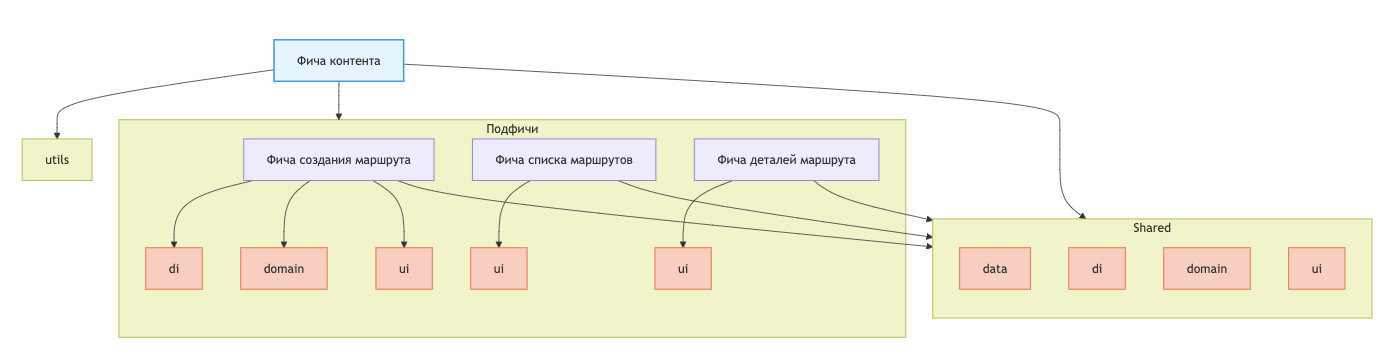
\includegraphics[height=0.4\textwidth]{Images/mobile_logic/структура_фичи.png}
\end{center}
\caption{Схема фичи контента приложения}
\label{fig:db_scheme}
\end{figure}
\end{landscape}

\subsection*{5.2 Реализация слоя данных (взаимодействия с бекендом)}
\addcontentsline{toc}{subsection}{5.2 Реализация слоя данных (взаимодействия с бекендом)}
Взаимодействие с бекендом было организовано в отдельном слое - слое данных, который у каждой фичи свой, что следует feature-first подходу. Кроме того, сами запросы отправляются через отдельные классы, которые были названы ApiClient, следуя логике, что эти классы отвечают за взаимодействие с API. А обработка исключений из этих классов была вынесены в классы, которые мы назвали, также согласно чистой архитектуре Repositories (репозиториями). Конкретную реализацию дата слоя фичи контента можно рассмотреть на примере классов \texttt{ContentApiClient} и \texttt{ContentApiClientImpl}. Эти классы отвечают за взаимодействие с API бекенда, предоставляя методы для получения маршрутов, фильтров, загрузки изображений, а также создания мест и маршрутов. Подробный код представлен в Приложении А, файл \texttt{content\_api\_client.dart}.

Так был создан ContentApiClient, который отвечает за взаимодействие с сервисом контента бекенда. Кроме того, следуая принципам ООП была сделана абстракция и имплементация клиента апи. Апи контента имеет 5 основных методов:

\begin{enumerate}
    \item \textbf{getRoutes} отвечает за получение списка маршрутов согласно выбранным пользователем фильтрам
    \item \textbf{getRoutesFilter} возвращает фильтров для выбора пользователем
    \item \textbf{uploadImages} позволяет загружать изображения пользователем на сервер
    \item \textbf{createPlace} отправляет запрос на создание пользвателем места маршрута
    \item \textbf{createRoute} позволяет создать маршрут
\end{enumerate}

Важно отметить, что апи слой не обрабатывает исключения, а отвечает только за передачу данных на следующий слой. Этим слоем в нашем приложении является репозиторий, а конкретно в случае фичи контента \texttt{ContentRepository} и его реализация \texttt{ContentRepositoryImpl}. Репозиторий инкапсулирует логику получения данных от API клиента, их преобразования в модели приложения и обработку исключений. Реализацию можно увидеть в Приложении А, файл \texttt{content\_repository.dart}.

Также была сделана абстракция репозитория, следуя принципам чистой архитектуры, также уже в репозитории происходит обработка исключений, которые может возвратить grpc. Для обработки исключений были созданы кастомные исключения (\texttt{AlreadyExistsGrpcException}, \texttt{InvalidArgumentGrpcException}, \texttt{InternalServerGrpcException}, \texttt{UnknownGrpcException}), наследуемые от \texttt{BaseGrpcException}. Маппинг стандартных \texttt{GrpcError} на эти кастомные исключения происходит с помощью расширения \texttt{GrpcErrorToException}. Код данных исключений и расширения доступен в Приложении А, файл \texttt{grpc\_exceptions.dart}.

Дальше полученные данные обрабатываются в соответствуюших BLoC-ах.

\subsubsection*{Получение списка маршрутов и применение фильтров}

Получение маршрута происходит через \texttt{RoutesBloc}. У него есть четыре состояния: \texttt{RoutesLoadSuccess} (успешная загрузка), \texttt{RoutesInitial} (начальное), \texttt{RoutesLoadInProgress} (загрузка) и \texttt{RoutesLoadFailure} (ошибка). Описание этих состояний находится в Приложении А, файл \texttt{routes\_state.dart}.

Этот блок обрабатывает одно событие \texttt{RoutesFetched}, сигнализирующее о необходимости загрузить список маршрутов. Код события представлен в Приложении А, файл \texttt{routes\_event.dart}.

Сама логика обработки события \texttt{RoutesFetched} и преобразования состояний происходит в \texttt{RoutesBloc}. Он взаимодействует с \texttt{ContentRepository} для получения данных. Полный код блока доступен в Приложении А, файл \texttt{routes\_bloc.dart}.

Так как событие всего одно, то для его обработки нужен только один метод \_onGetRoutes

Для получения фильтра маршрутов был создан \texttt{FilterRoutesBloc}, у которого четыре состояния: \texttt{FilterRoutesInitial}, \texttt{FilterRoutesLoadInProgress}, \texttt{FilterRoutesLoadSuccess} (успешная загрузка доступных и пользовательских фильтров) и \texttt{FilterRoutesLoadFailure}. Код состояний можно найти в Приложении А, файл \texttt{filter\_routes\_state.dart}.

Этот блок обрабатывает уже два события: \texttt{AvailableFilterRoutesFetched} (запрос доступных фильтров) и \texttt{UserFilterRoutesChanged} (изменение пользовательских фильтров). Код событий представлен в Приложении А, файл \texttt{filter\_routes\_event.dart}.

Логика обновления состояния для \texttt{FilterRoutesBloc} описана в соответствующем файле. Блок обрабатывает события получения доступных фильтров и изменения пользовательских фильтров, взаимодействуя с \texttt{ContentRepository}. Код блока находится в Приложении А, файл \texttt{filter\_routes\_bloc.dart}.

При этом обновление списка маршрутов происходит при изменении пользователем фильтров с помощью механизма \texttt{BlocListener} в виджете \texttt{ContentPage}. При изменении фильтров в \texttt{FilterRoutesBloc}, инициируется событие \texttt{RoutesFetched} в \texttt{RoutesBloc}. Код данного слушателя представлен в Приложении А, файл \texttt{content\_page\_listener.dart}.

\subsubsection*{Создание маршрута}
Фича создания маршрутов является более сложной фичой, чем фичи получения и фильтрацию, потому что в ней сосредоточено сразу несколько других фичей:

\begin{itemize}
    \item Взаимодействие с плагином Яндекс.Карт, чтобы пользователь мог выбрать точку маршрута на карте
    \item Валидация всех полей при заполнении маршрута
    \item Возможность изменять порядок мест маршрута перетаскиванием на странице создания
    \item Правильная последовательность отправки запросов на бекенд. Потому что сначала нужно отправить запрос на создание места, потом на создание фотографий и только потом создать маршрут
\end{itemize}

Для реализации этой сложной части нами было выделено 3 блока и 1 интерактор для связи этих блоков между собой.

Так как у нас есть две страницы для создания маршрута, было решено для каждой страницы сделать свой блок, чтобы перейти на следующую страницу можно было только при правильном заполнении данных на предыдущей. 

Так для  заполнения общей информации о маршруте был создан \texttt{CreateRouteFormBloc}. У него есть два основных состояния: \texttt{CreateRouteFormEdited} (форма редактируется) и \texttt{CreateRouteFormFilled} (форма заполнена корректно). Эти состояния содержат поля для общей информации о маршруте. Код состояний представлен в Приложении А, файл \texttt{create\_route\_form\_state.dart}.

\texttt{CreateRouteFormBloc} обрабатывает события для обновления каждого поля формы (название, описание, тип транспорта и т.д.), а также событие для сброса формы. Код событий представлен в Приложении А, файл \texttt{create\_route\_form\_event.dart}.

и сама логика обработки событий и обновления состояния определена в \texttt{CreateRouteFormBloc}. Блок управляет состоянием формы создания общей информации о маршруте и определяет, заполнена ли форма корректно. Полный код представлен в Приложении А, файл \texttt{create\_route\_form\_bloc.dart}.

За создание и изменение порядка точек на маршруте отвечает \texttt{CreatePointsFormBloc}. У него есть одно состояние \texttt{CreatePointsFormState}, содержащее список моделей точек маршрута (\texttt{CreatePointFormModel}). Код состояния представлен в Приложении А, файл \texttt{create\_points\_form\_state.dart}.

И этот блок обрабатывает события добавления (\texttt{PlaceFormAddPoint}), обновления (\texttt{PlaceFormUpdatePoint}), удаления (\texttt{PlaceFormDeletePoint}) точки, изменения порядка точек (\texttt{PlaceFormReorderPoints}), а также сброса формы (\texttt{PlaceFormReset}). Код событий представлен в Приложении А, файл \texttt{create\_points\_form\_event.dart}.

Сама логика обновления состояния и обработки событий описана в \texttt{CreatePointsFormBloc}. Блок управляет списком точек маршрута. Полный код представлен в Приложении А, файл \texttt{create\_points\_form\_bloc.dart}.

Кроме того, есть блок \texttt{CreatePointFormBloc}, который отвечает за редактирование точки маршрута на самой странице. Он имеет состояния для управления формой редактирования отдельной точки маршрута, такие как \texttt{CreatePathPointEditedFormModel}, \texttt{CreatePathPointFilledFormModel}, \texttt{CreatePlacePointEditedFormModel}, и \texttt{CreatePlacePointFilledFormModel}. Код состояний представлен в Приложении А, файл \texttt{create\_point\_form\_state.dart}.

А также он содержит следующие события на изменения этого состояния. Код событий представлен в Приложении А, файл \texttt{create\_point\_form\_event.dart}.

Сама логика обработки происходит в блоке \texttt{CreatePointFormBloc}. Он управляет состоянием формы редактирования отдельной точки маршрута, обрабатывает события обновления полей, управляет изображениями и определяет, заполнена ли форма точки корректно. Полный код представлен в Приложении А, файл \texttt{create\_point\_form\_bloc.dart}.

Объединение состояния блоков \texttt{CreatePointsFormBloc} и \texttt{CreateRouteFormBloc}  происходит в методе \texttt{createRoute} интерактора \texttt{CreateRouteInteractor}. Интерактор координирует процесс создания маршрута, взаимодействуя с \texttt{ContentRepository}. Полный код представлен в Приложении А, файл \texttt{create\_route\_interactor.dart}.

В рамках главы 4 была детально описана реализация слоя логики мобильного приложения "Путешествия по России" с применением архитектурного паттерна BLoC (Business Logic Component). Были разработаны отдельные BLoC'и для управления состоянием различных функциональных модулей, таких как получение и фильтрация списка маршрутов (RoutesBloc, FilterRoutesBloc), а также для сложной фичи создания маршрутов.   

Для реализации функционала создания маршрутов были выделены блоки CreateRouteFormBloc  для управления общей информацией о маршруте и CreatePointsFormBloc  для работы со списком точек маршрута, включая изменение их порядка. Отдельный блок CreatePointFormBloc  был разработан для редактирования информации по конкретной точке маршрута, учитывая различные типы точек (опорная точка или место).   

Взаимодействие между блоками CreatePointsFormBloc и CreateRouteFormBloc, а также координация отправки запросов к слою данных, реализованы в интеракторе CreateRouteInteractor, который обеспечивает правильную последовательность операций, включая создание мест и загрузку изображений перед созданием самого маршрута.   

Таким образом, в главе 4 продемонстрирован подход к разработке мобильного приложения с четким разделением ответственности между компонентами с использованием BLoC и интеракторов, что способствует модульности, тестируемости и поддерживаемости кода.


